\section{Overview}

\subsection{Overview and Original Design}

The LTCC consists of six identical sectors, each containing:

\begin{itemize}
	\item 108 lightway adjustable mirrors
	\item 36 Winston light collecting Cones
	\item 36 5’’ Photonis X4500B PMT
	\item 36 Magnetic Shields
	\item C4F10 Gas, refraction index: 1.00134
\end{itemize}


The optics of each y module was designed to focus the light onto a photomultiplier tube (PMT) associated with that module and located in the region obscured by the coils.
Fig.~\ref{fig:optics} shows the optical arrangement of one module. The array of the modules in one sector is shown in Fig.~\ref{fig:ltccArray}.

\begin{figure}[hbt]
	\centering
	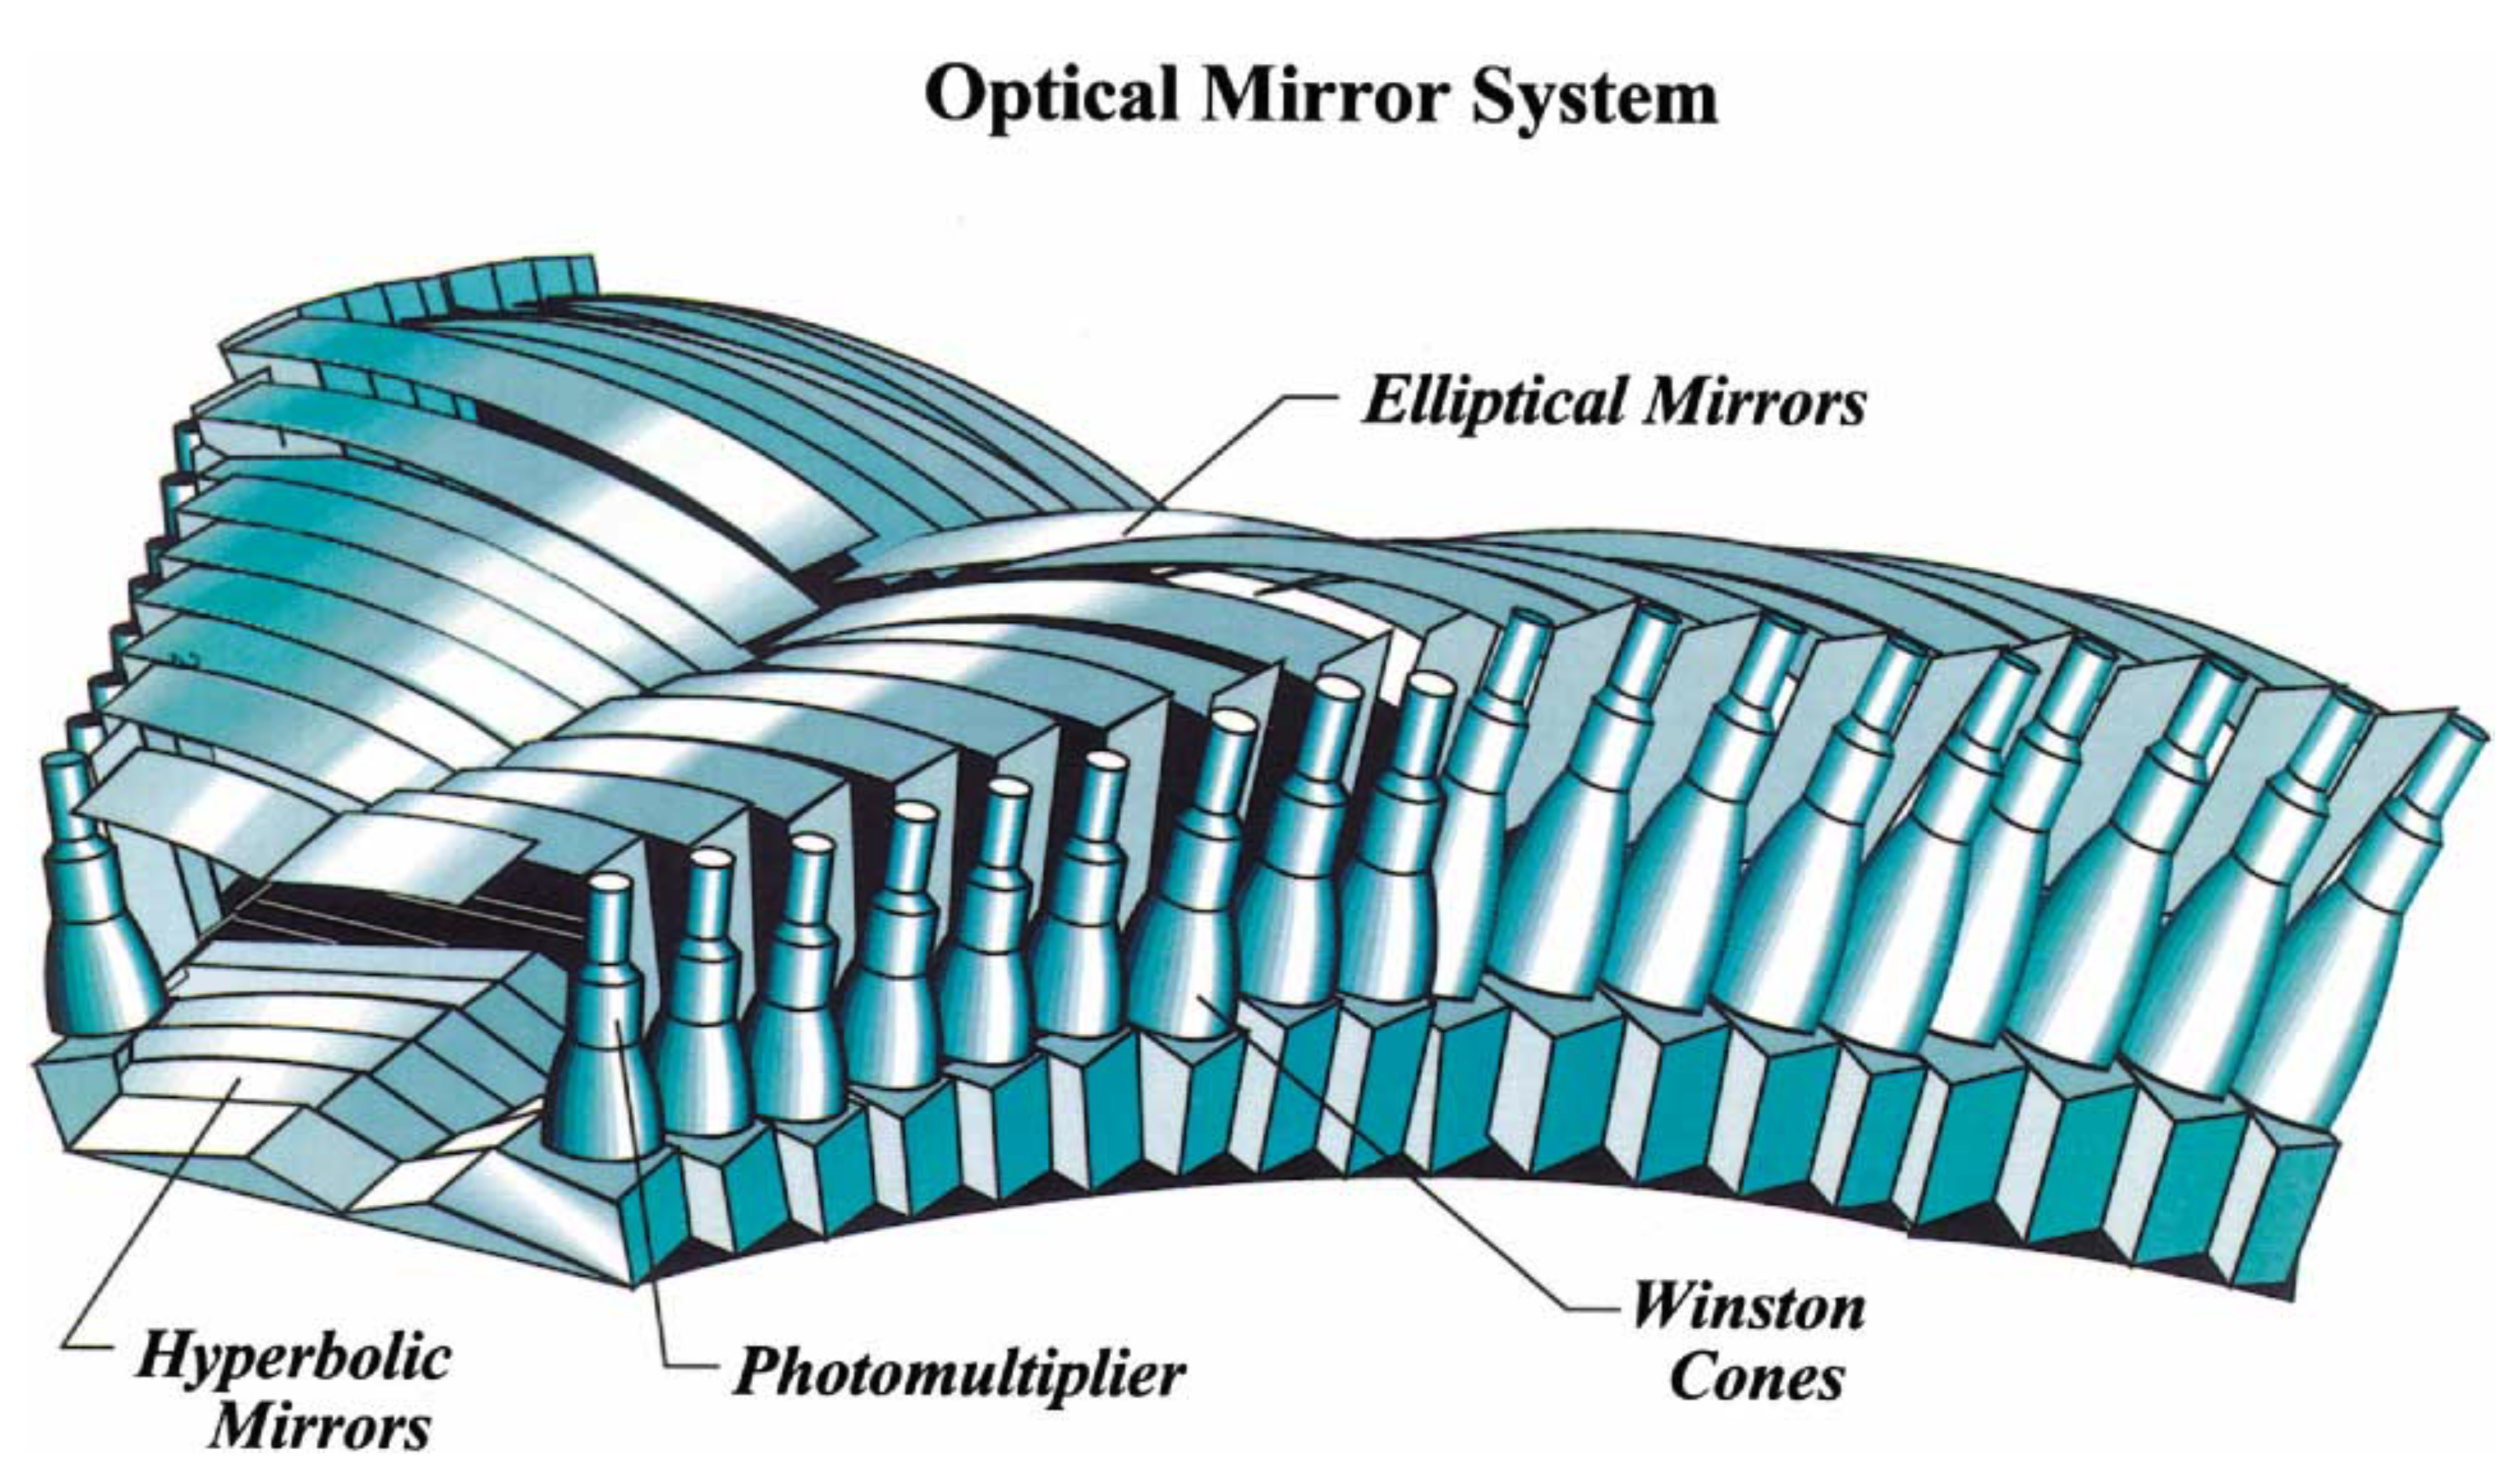
\includegraphics[width=1.0\columnwidth,keepaspectratio]{img/ltccArray.png}
	\caption{A schematic diagram of the array of optical modules in one of the six sectors.}
	\label{fig:ltccArray}
\end{figure}
